\documentclass{article}
\usepackage[top=1cm, bottom=1.5cm, left=1.5cm, right=1.5cm]{geometry}
\usepackage{hyperref}
\usepackage{mdframed}
\usepackage[svgnames]{xcolor}
\usepackage{multicol}
\usepackage{changepage}
\usepackage{fontawesome5}
\usepackage{tikz}
\usepackage{graphicx}
\usepackage{lmodern}

\definecolor{skyblue}{RGB}{70, 136, 160}

\hypersetup{
    colorlinks=false,
    linkcolor=blue,
    urlcolor=blue,
    citecolor=blue,
    pdfborderstyle={/S/U/W 0}
}

\begin{document}
\pagenumbering{gobble}

\begin{adjustwidth}{-2cm}{-1.6cm}
    \begin{mdframed}[backgroundcolor=skyblue!20, frametitlebackgroundcolor=skyblue!20]
        \begin{adjustwidth}{1cm}{1cm}
            \section*{\hspace*{0.6cm}\fontsize{24}{24}\selectfont\textbf{Md. Abdullah Al Mamun}}
            \begin{itemize}
                \item[] \faEnvelope\ Email\hspace{0.4cm}: \href{mailto:md.abdullahalmamun.shohag.abd@gmail.com}{md.abdullahalmamun.shohag.abd@gmail.com}
                \item[] \faPhone\ Phone\hspace{0.35cm}: \href{tel:+8801792760883}{+880 1792 760883}
                \item[] \faMapMarker\ Address\hspace{0.17cm}: Motihar Thana, Rajshahi 6204
            \end{itemize}
            \begin{tikzpicture}[remember picture,overlay]
                \node[anchor=north east, inner sep=0pt] at (current page.north east) [xshift=-1.2cm, yshift=-0.4cm] {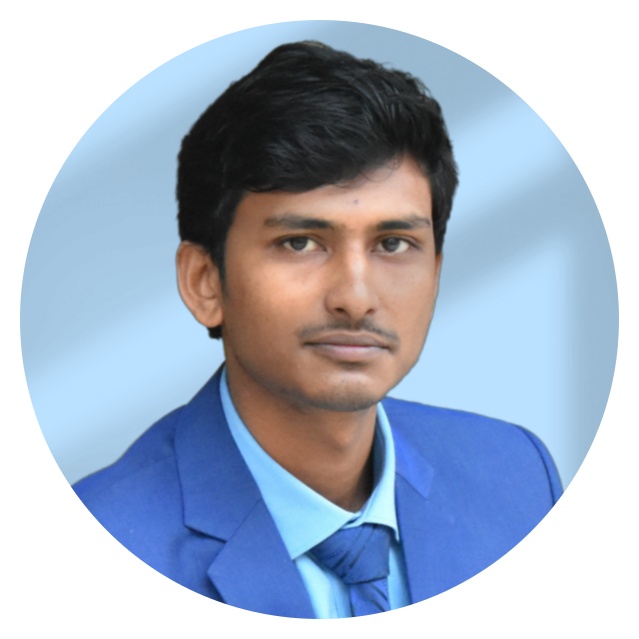
\includegraphics[width=5cm]{profile-pic2_1.png}};
            \end{tikzpicture}
        \end{adjustwidth}
    \end{mdframed}

\end{adjustwidth}

\begin{adjustwidth}{0cm}{0cm}
    \vspace{0.5cm}
    \begin{multicols}{2}
        \section*{Objectives}
        I am known for technical expertise and exceptional project management, marked by a supportive approach.
        My fervent passion for technology keeps me attuned to emerging trends. I aim to blend advanced technology with human aspiration, driving innovative, transformative changes. My vision is focused on pioneering progress, steering the world towards an era marked by unprecedented technological advancements, and fostering an environment where innovation and human potential synergize seamlessly.

        \section*{Skill Highlights}
        \subsection*{Technical Skills}
        \begin{itemize}
            \item Project Management
            \item Software Development
            \item Robotics: Arduino
            \item Web Development: DJango, NodeJS, React
            \item Programming Languages: \\
                  C, C++, Python, JavaScript, Java, MATLAB
            \item Office/Excel: LibreOffice, Microsoft Office
        \end{itemize}
        \subsection*{Interpersonal Skills}
        \begin{itemize}
            \item Technological Adaptation
            \item Event Management
            \item Problem Solving
            \item Communication
            \item Teamwork
        \end{itemize}

        \section*{Experiences}
        \subsection*{Project Management}
        \begin{itemize}
            \item \textbf{SuggestBot-BN}, Developer (December 2020)\\
                  A Bengali Wikipedia bot that suggests articles based on users' edit history
            \item \textbf{Ubuntu Touch}, Contributor (Jun 2021 to Present)\\
                  Test segment and development on Redmi 9 (Lancelot)
            \item \textbf{SimpleNeuralNetwork}, Developer (September 2023)\\
                  A simple integration of Neural Network Model detecting safe and poisonous food\\
                  Embedded System, UBports
            \item \textbf{Halium Project}, Contributor (January to March 2021)\\
                  Collaborated with a Jolla Software Engineer called Nikita Ukhrenkov (nikita.ukhrenkov@jolla.com)
            \item \textbf{QuinX}, Developer (December 2022)\\
                  An autonomous line follower robot designed with Arduino Mega 2560 to track and follow a predefined path on a surface
        \end{itemize}

        \subsection*{Volunteering}
        \begin{itemize}
            \item \textbf{8th RCF Career Fair}, RUET Career Forum, Human Resource Management (September, 2023)
        \end{itemize}

        \section*{Education}
        \begin{itemize}
            \item \textbf{Bachelor of Science in Engineering: Computer Science and Engineering} - (4th Semester, CGPA-3.36 (upto 1st Semester), 2020–21), Rajshahi University of Engineering and Technology, Rajshahi
            \item \textbf{Higher School Certificate (HSC): Science} (GPA-5.00, 2019–20), Police Lines School and College, Rangpur
            \item \textbf{Secondary School Certificate (SSC): Science} (GPA-5.00, 2017–18), Gangachara Adarsha High School, Gangachara, Rangpur
        \end{itemize}

        \section*{Languages}
        \begin{itemize}
            \item English – Fluent
            \item Bengali – Native
        \end{itemize}

        \section*{References}
        \begin{itemize}
            \item \textbf{Md. Azmain Yakin Srizon}, Lecturer, Department of CSE, RUET, Email: \href{mailto:azmainsrizon@cse.ruet.ac.bd}{azmainsrizon@cse.ruet.ac.bd}
            \item \textbf{Nikita Ukhrenkov}, Senior Software Developer, Jolla Ltd., Philippines, Email: \href{mailto:nikita.ukhrenkov@jolla.com}{nikita.ukhrenkov@jolla.com}
        \end{itemize}

        \section*{External Links}
        \begin{itemize}
            \item \textbf{GitHub Profile:} \href{https://github.com/HackerShohag}{https://github.com/HackerShohag}
            \item \textbf{Portfolio Website:} \href{https://hackershohag.github.io}{https://hackershohag.github.io}
            \item \textbf{Linked-In:} \href{https://www.linkedin.com/in/hackershohag}{https://www.linkedin.com/in/hackershohag}
        \end{itemize}
    \end{multicols}
\end{adjustwidth}

\end{document}
